Kiểm thử phần mềm là một bước quan trọng trong quy trình phát triển phần mềm, đảm bảo sản phẩm đáp ứng đầy đủ, chính xác những yêu cầu của khách hàng, giúp nhà phát triển phát hiện ra các lỗi tiềm ẩn, giảm thiểu các rủi ro và chi phí phát sinh trong quá trình bảo dưỡng và nâng cấp phần mềm trong tương lai.\\
\begin{enumerate}
    \item \textbf{Chức năng đăng ký tài khoản}
    \begin{table}[H]
\centering
\scalebox{0.65}{
\begin{tabular}{|p{1cm}|p{9cm}|p{9cm}|p{2cm}|}
\hline
STT & Mô tả test-case & Kết quả mong muốn & Kết luận \\ \hline
1 & Đăng ký tài khoản với email là dhmt7210@gmail.com, nhập tên là Trí, nhập họ là Đặng, nhập mật khẩu, nhập lại mật khẩu, nhập ngày sinh, nhập địa chỉ, nhấn đăng ký & Đăng ký thành công, chuyển đến trang đăng nhập & PASS \\ \hline
2 & Đăng ký tài khoản với email đã tồn tại & Báo lỗi đã tồn tại email & PASS \\ \hline
3 & Đăng ký tài khoản với tên trống & Báo lỗi yêu cầu nhập tên & PASS \\ \hline
\end{tabular}}
\end{table}
\item \textbf{Chức năng trên Plan}
\begin{table}[H]
\centering
\scalebox{0.65}{
\begin{tabular}{|p{1cm}|p{9cm}|p{9cm}|p{2cm}|}
\hline
STT & Mô tả test-case & Kết quả mong muốn & Kết luận \\ \hline
1 & Bấm chọn tạo Plan mới. Chọn thời gian bắt đầu là 10/11/2021, thời gian kết thúc là 14/11/2021, nhấn Create & Chuyển trang đến List Plan & PASS \\ \hline
2 & Chọn giờ và tạo các activity trong ngày. Chọn activity, Hotel (check in),Eat n Drink, Attraction, bấm CREATE&Hiển thị thông báo thành công& PASS \\ \hline
3 & Kiểm tra tạo nhiều activity trùng giờ&Hiển thị thông báo trùng thời gian &  PASS \\ \hline
4 & Tìm kiếm kế hoạch muốn tham khảo, bấm vào ô tìm kiếm và nhập tên địa điểm và nhấn "CREATE"&Hiển thị danh sách kế hoạch có tên địa điểm đã nhập &  PASS \\ \hline
5 & Xem kế hoạch có sẵn &Hiển thị kế hoạch đã có &  PASS \\
\hline
6 & Chia sẻ kế hoạch với bạn bè, tại trang danh sách kế hoạch đã tạo nhấn Share cho bạn bè &Hiển thị thông báo thành công&  PASS \\ \hline
7 & Xóa kế hoạch đã tạo & Hiển thị thông báo thành công & PASS \\
\end{tabular}}
\end{table}
\item \textbf{Chức năng tạo bài review sau chuyến đi}
\begin{table}[H]
\centering
\scalebox{0.65}{
\begin{tabular}{|p{1cm}|p{9cm}|p{9cm}|p{2cm}|}
\hline
STT & Mô tả test-case & Kết quả mong muốn & Kết luận \\ \hline
1 & Bấm vào biểu tượng tạo bài Blog, nhấp bài viết, upload hình ảnh và nhấn "Create" & Thông báo tạo bài Blog thành công & PASS \\ \hline
2 & Bấm vào biểu tượng bạn bè hoặc thông báo, Bấm "Accecpt" để đồng ý kết bạn&Hiển thị thông báo thành công& PASS \\ \hline
3 & Bấm vào biểu tượng bạn bè hoặc thông báo, Bấm "Decline" để từ chối kết bạ & Hiển thị thông báo thành công &  PASS \\ \hline
4 & Bấm vào biểu tượng bạn bè hoặc tìm kiếm bạn bè muốn Unfriend, bấm Unfriend & Hiển thị thông báo thành công  &PASS \\ \hline
\end{tabular}}
\end{table}

\item \textbf{Chức năng kết bạn}
\begin{table}[H]
\centering
\scalebox{0.65}{
\begin{tabular}{|p{1cm}|p{9cm}|p{9cm}|p{2cm}|}
\hline
STT & Mô tả test-case & Kết quả mong muốn & Kết luận \\ \hline
1 & Bấm tìm kiếm bạn bè, chọn bạn bè muốn kết bạn bấm AddFriend & Thông báo gởi lời mời kết bạn thành công & PASS \\ \hline
2 & Bấm vào biểu tượng bạn bè hoặc thông báo, Bấm "Accecpt" để đồng ý kết bạn&Hiển thị thông báo thành công& PASS \\ \hline
3 & Bấm vào biểu tượng bạn bè hoặc thông báo, Bấm "Decline" để từ chối kết bạ & Hiển thị thông báo thành công &  PASS \\ \hline
4 & Bấm vào biểu tượng bạn bè hoặc tìm kiếm bạn bè muốn Unfriend, bấm Unfriend & Hiển thị thông báo thành công  &PASS \\ \hline
\end{tabular}}
\end{table}
\item \textbf{Chức năng trò chuyện}
\begin{table}[H]
\centering
\scalebox{0.65}{
\begin{tabular}{|p{1cm}|p{9cm}|p{9cm}|p{2cm}|}
\hline
STT & Mô tả test-case & Kết quả mong muốn & Kết luận \\ \hline
1 & Bấm tìm kiếm bạn bè, chọn bạn bè muốn trò chuyện, nhập thông tin hội thoại và bấm "Gửi" & Thông báo gởi thành công & PASS \\ \hline

\end{tabular}}
\end{table}
\end{enumerate}








% Các công nghệ sử dụng trong kiểm thử thử hệ thống:
% \begin{center}
%   \captionsetup{type=figure}
%   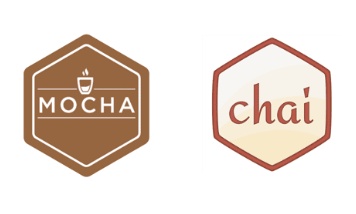
\includegraphics[width=10cm]{image/mocha_chai.png}
%   \captionof{figure}{Mocha framework và Chai assertion library}
% \end{center}

% Mocha là một Javascript framework kiểm thử chạy trên Node.js và trình duyệt, giúp cho việc kiểm tra bất đồng bộ một cách đơn giản. Mocha được đánh giá là một framework kiểm thử đơn giản, linh hoạt và chạy ổn định. Hiện nay, Mocha được nhiều công ty lớn sử dụng trong kiểm thử hệ thống.

% Chai là một thư viện assertion với nhiều tuỳ chọn cho phép kiểm tra đối tượng như "should", "expect" và "assert". Trong hệ thống Tổ chức-Hành chính, nhóm nhận thấy có nhiều API có phương thức GET trả về dữ liệu dưới dạng JSON nên nhóm sử dụng Chai để thực hiện HTTP request và kiểm tra các giá trị trả về.

% Chương kiểm thử sẽ liệt kê các phương pháp nhóm sử dụng để kiểm thử, kiểm tra các chức năng của hệ thống trước khi đưa ra thực tế.
% \clearpage
% \section{Kiểm thử đơn vị - Unit test}
% Quá trình hiện thực hệ thống sử dụng Mocha framework để tiến hành kiểm thử đơn vị. 
% Kiểm thử đơn vị được tiến hành trên các thư viện, hàm chức năng đơn lẻ. Cụ thể đoạn code phía dưới kiểm thử một chức năng về xử lý chuỗi ký tự.
% \begin{lstlisting}
% var T = require('./common.js');
% var assert = require('assert');
% describe('Test T.dateToText', function () {
%     it('test T.dateToText(dd/mm/yyyy)', function () {
%         assert.equal(T.dateToText(new Date().getTime(), 'dd/mm/yyyy'), '13/09/2020');
%     });
%     it('test T.dateToText(mm/yyyy)', function () {
%         assert.equal(T.dateToText(new Date().getTime(), 'mm/yyyy'), '09/2020');
%     });
%     it('test T.dateToText(yyyy)', function () {
%         assert.equal(T.dateToText(new Date().getTime(), 'yyyy'), '2020');
%     });
%     it('test nextYear', function () {
%         assert.equal(T.dateToText(Date.nextYear(), 'yyyy'), '2021');
%     });
%     it('test lastYear', function () {
%         assert.equal(T.dateToText(Date.lastYear(), 'yyyy'), '2019');
%     });

%     describe('Test T.validateEmail', function () {
%         it('test T.validateEmail', function () {
%             assert.equal(T.validateEmail('luanvantotnghiep@aao.hcmut.edu.vn'), true);
%         });
%         it('test T.validateEmail', function () {
%             assert.equal(T.validateEmail('luanvantotnghiep@.hcmut.edu.vn'), false)
%         });
%     });

%     describe('Test string methods', function () {
%         it('test upper first char', function () {
%             assert.equal('node.js'.upFirstChar(), 'Node.js')
%         });
%         it('test lower first char', function () {
%             assert.equal('node.js'.upFirstChar().lowFirstChar(), 'node.js');
%         });
%     });
% });
% \end{lstlisting}
% \clearpage
% Thu được kết quả thực thi lúc kiểm thử như sau:
% \begin{figure}[H]
%   \centering
%   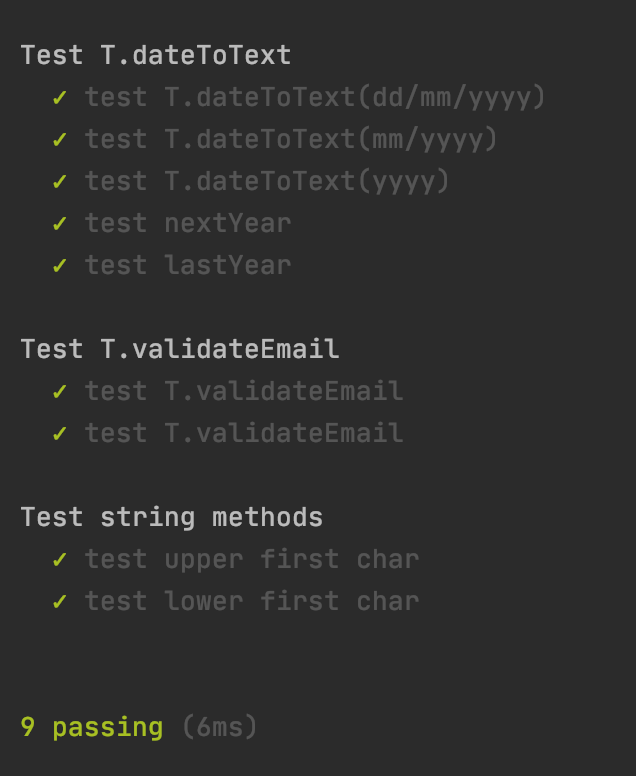
\includegraphics[width=5cm]{image/unitest.png}
%   \caption{Kết quả chạy một số đoạn kiểm thử ở mức kiểm thử đơn vị}
%   \label{fig:npm_run_test_unit1}
% \end{figure}

% \section{Kiểm thử tích hợp (Integration Test)}
% Ở mức kiểm thử tích hợp giúp phát hiện lỗi giao tiếp giữa các thành phần với nhau. Cụ thể, ở chương trình hiện tại giao tiếp giữa các phần controller với model, view và controller là phần quan trọng nhất.

% Việc kiểm thử tích hợp mất khá nhiều thời gian và rất phức tạp, để trình bày hết ở báo cáo này cũng rất khó. Ví dụ kiểm thử một vài chức năng thuộc phần giao tiếp giữa controller và model như sau:

% \begin{lstlisting}
% describe('Test API', function() {
%   it('Get page event:', function(done) {
%     chai.request(server)
%         .get('/api/event/page/1/50')
%         .end(function(err, res){
%           res.should.have.status(200);
%           res.should.be.json;
%           assert.equal(JSON.parse(res.text).error, null);
%           done();
%         });
%   });

%   it('Post event:' , function(done) {
%     chai.request(server)
%         .post('/api/event/default')
%         .send({thuTu: 4})
%         .end(function(err, res){
%           res.should.have.status(200);
%           res.should.be.json;
%           assert.equal(JSON.parse(res.text).error, null);
%           done();
%         });
%   });
% });
% \end{lstlisting}

% Thu được kết quả thực thi lúc kiểm thử như sau:
% \begin{figure}[H]
% 	\centering
% 	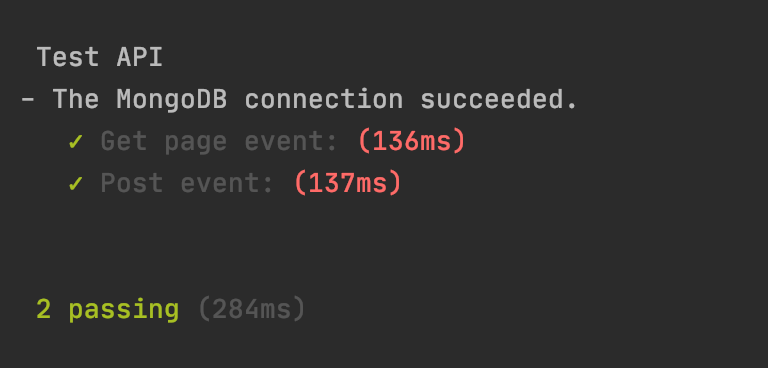
\includegraphics[width=7cm]{image/integrationtest.png}
% 	\caption{Kết quả chạy một số đoạn kiểm thử ở mức kiểm thử tích hợp}
% 	\label{fig:npm_run_test_unit2}
% \end{figure}

% \section{Kiểm thử hệ thống}
% Trong quá trình phát triển hệ thống, nhóm tiến hành kiểm tra các chức năng với dữ liệu mẫu từ khâu khởi tạo đến chạy thực tế. Cụ thể, phần này, nhóm 
% trình bày quá trình kiểm thử việc một sự kiện trên hệ thống, sinh viên đăng ký tham gia sự kiện và điểm danh sự kiện.

% \subsection{Tạo sự kiện, thêm sinh viên, điểm danh sự kiện}
% Trước khi sự kiện diễn ra, quản trị viên sẽ tạo sự kiện trên hệ thống, điền các thông tin liên quan đến sự kiện như mô tả, hình ảnh, thời gian, 
% số lượng sinh viên và các thông tin khác. Hình \ref{fig:eventAdmin} thể hiện sự kiện mới đã được tạo và kích hoạt trên hệ thống. Ngoài ra còn thực hiện quá trình chấm điểm rèn luyện.
% \begin{figure}[H]
%   \centering
%   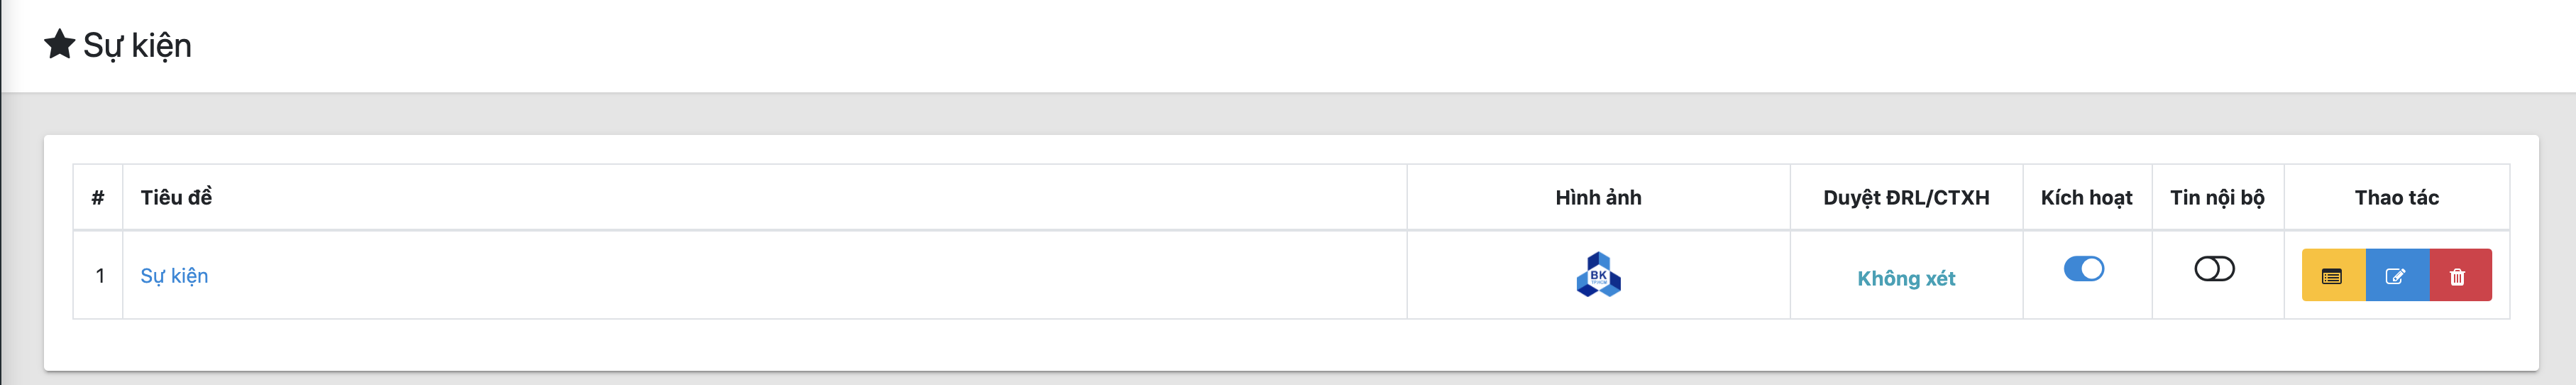
\includegraphics[width=\textwidth]{image/testing-event-admin.png}
%   \caption{Admin thêm sự kiện mới}
%   \label{fig:eventAdmin}
% \end{figure}
% Sau khi điền thông tin mô tả sự kiện, quản trị viên cần tạo câu hỏi đăng ký tham gia sự kiện để cho sinh viên có thể đăng ký tham gia, hình 
% \ref{fig:eventAdminAnswer} mô tả một câu hỏi trong \textbf{Sự kiện mới}, loại câu hỏi là Lựa chọn.
% \begin{figure}[H]
%   \centering
%   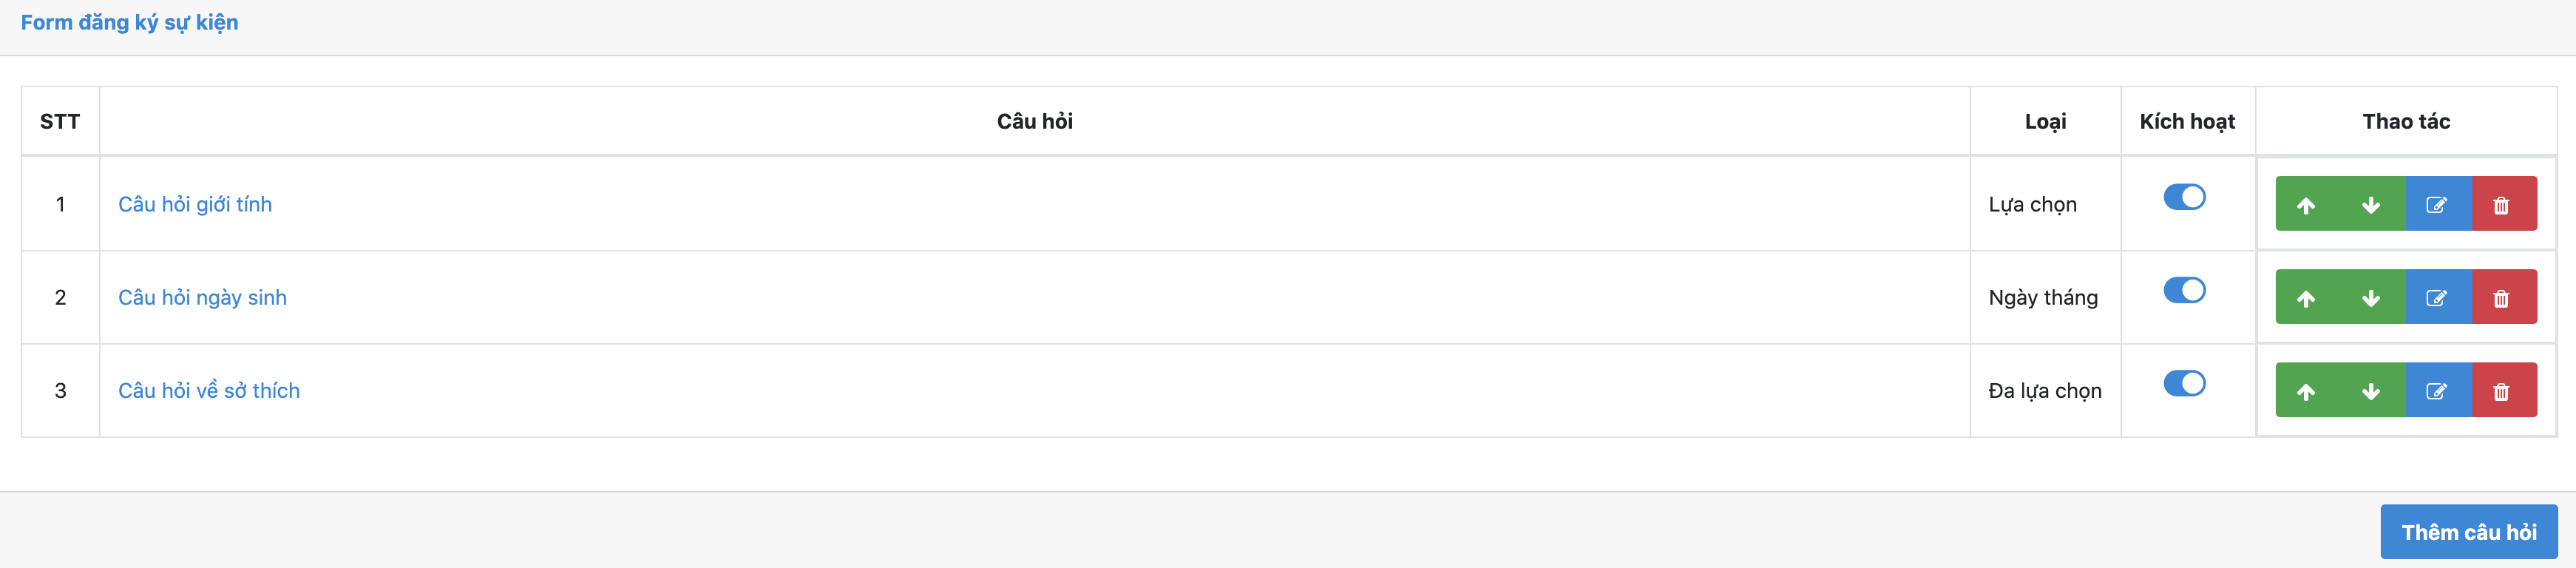
\includegraphics[width=\textwidth]{image/testing-event-answer.png}
%   \caption{Admin thêm câu hỏi cho sự kiện}
%   \label{fig:eventAdminAnswer}
% \end{figure}
% \clearpage
% Sau khi sự kiện được kích hoạt, quản trị viên điều chỉnh phần menu để các sự kiện có thể hiện lên trang tin tức. Hình \ref{fig:eventHome} thể hiện một sự kiện được đặt 
% trên trang tin tức, với nút đăng ký để sinh viên có thể lựa chọn đăng ký trực tiếp hoặc chọn vào sự kiện để xem thông tin chi tiết trước khi đăng ký.
% \begin{figure}[H]
%   \centering
%   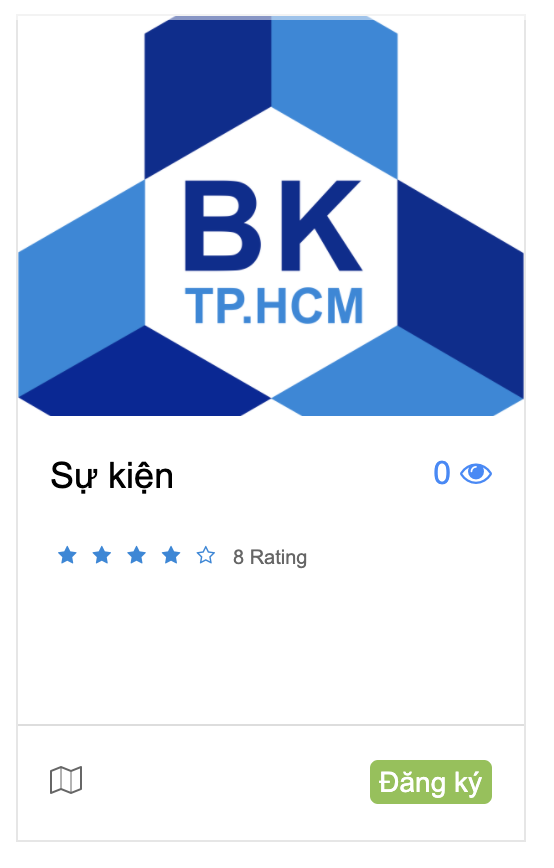
\includegraphics{image/testing-event-home.png}
%   \caption{Thông tin sự kiện trên trang thông tin tổng hợp}
%   \label{fig:eventHome}
% \end{figure}
% \clearpage
% Sau khi theo dõi thông tin và trả lời các câu hỏi liên quan đến sự kiện, sinh viên chọn nút đăng ký để đăng ký tham gia sự kiện. Mỗi sinh viên chỉ đăng ký một 
% lần duy nhất, như hình \ref{fig:eventRegister}
% \begin{figure}[H]
%   \centering
%   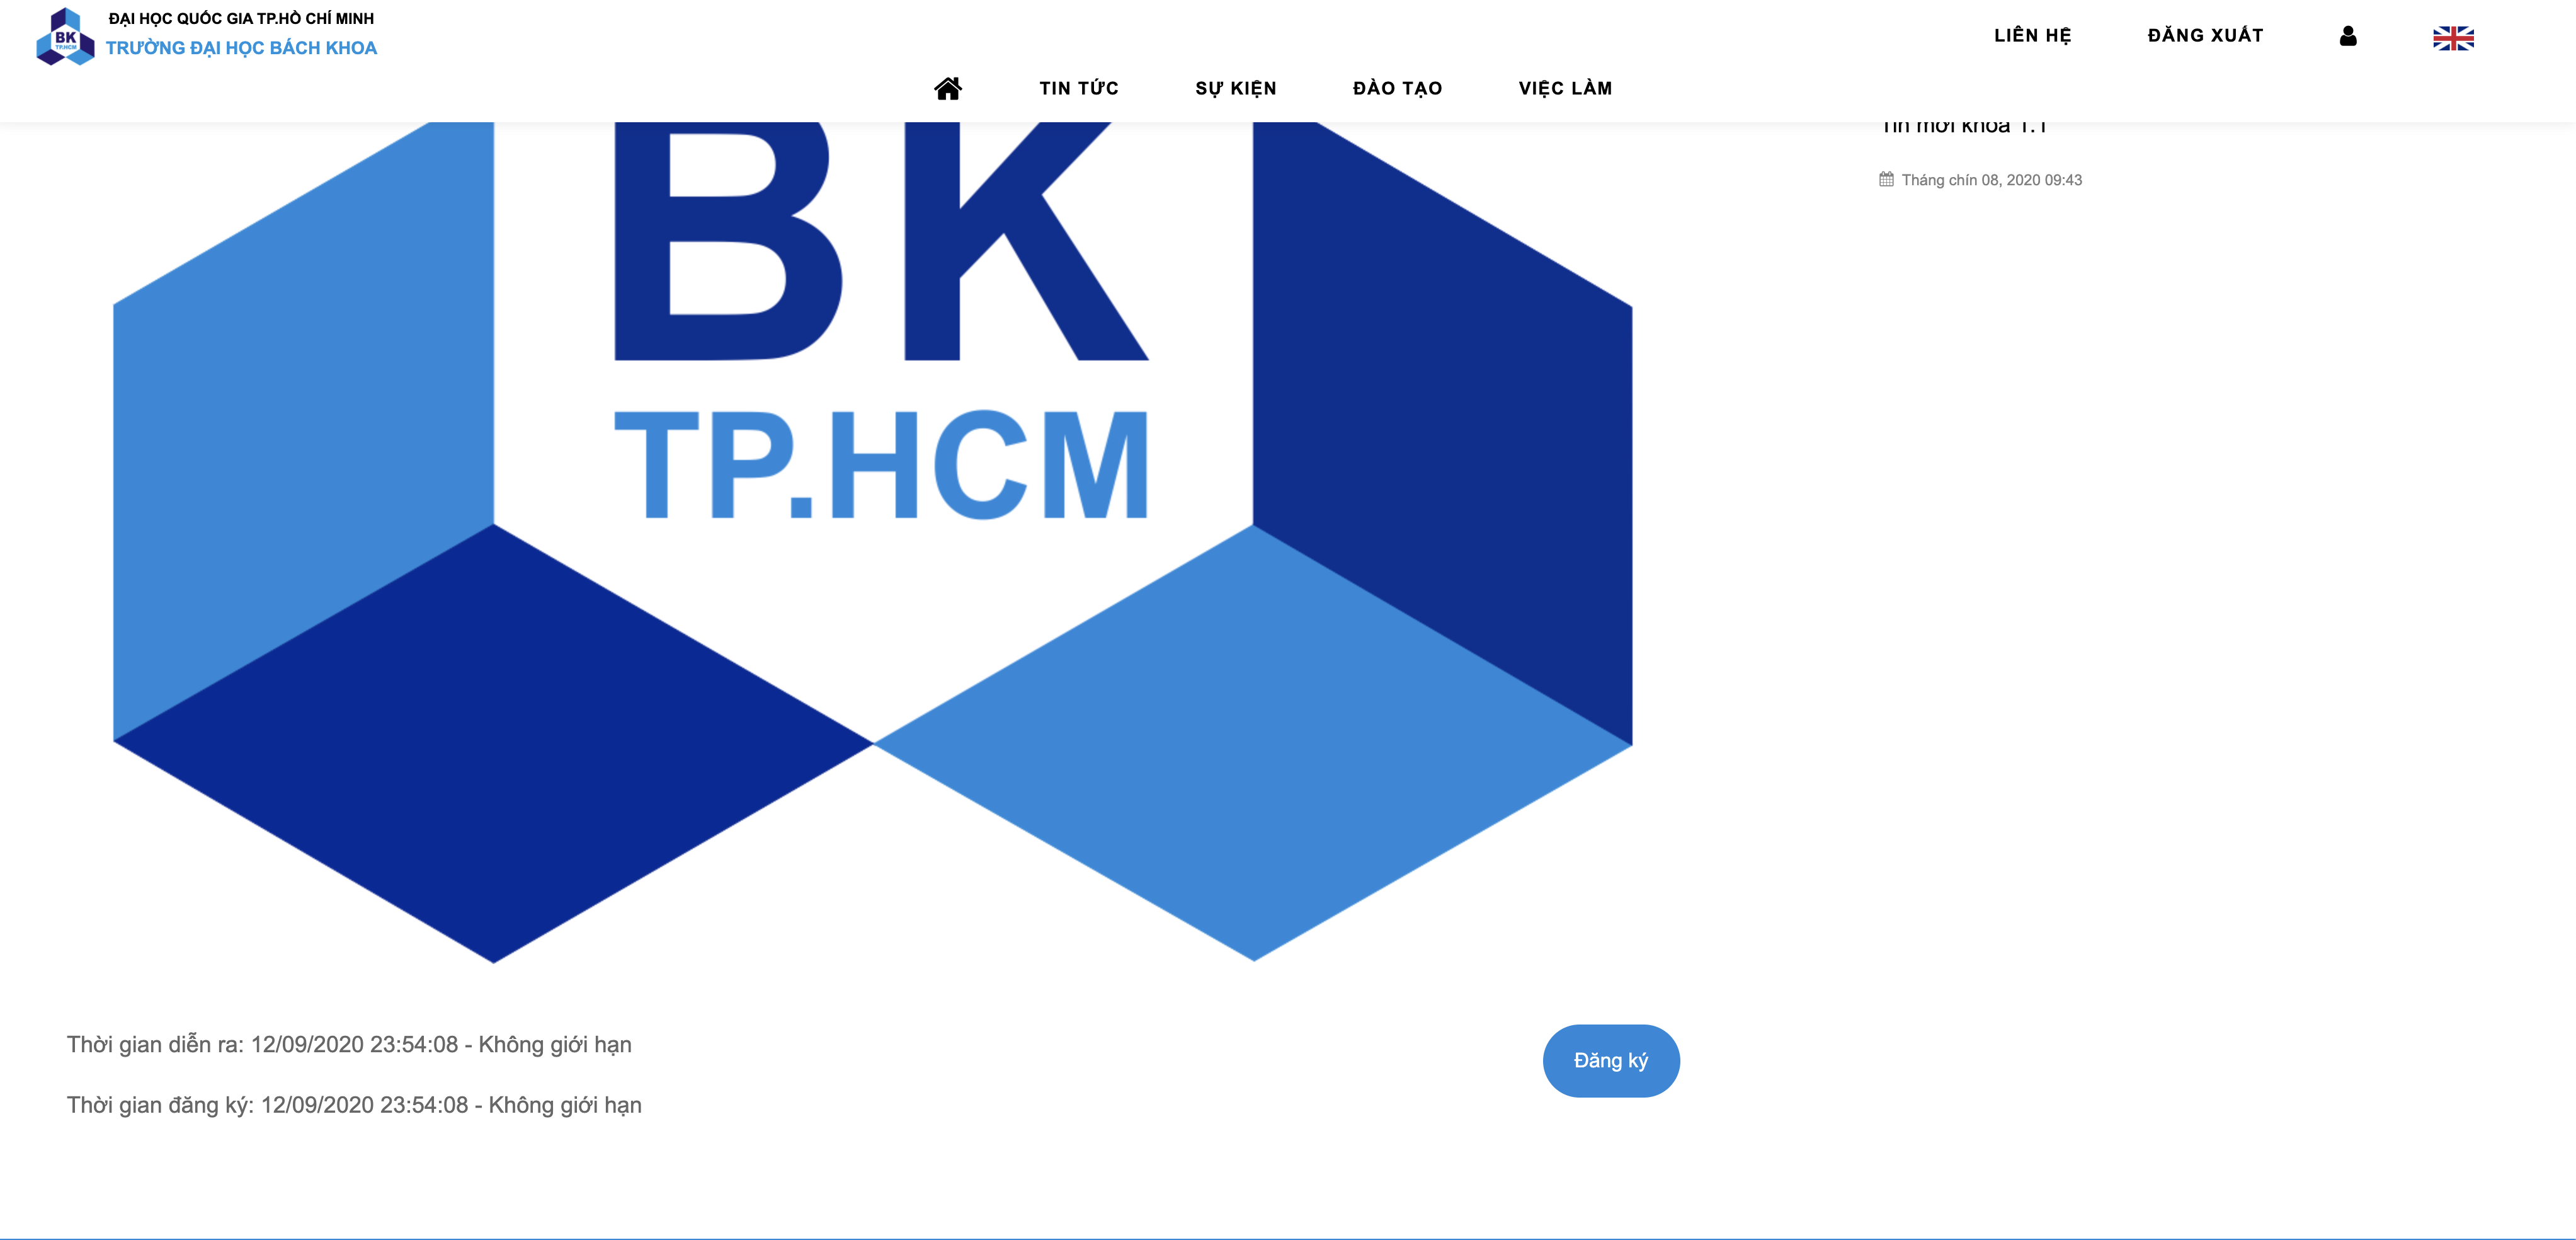
\includegraphics[width=\textwidth]{image/testing-event-register.png}
%   \caption{Sinh viên đã đăng ký sự kiện}
%   \label{fig:eventRegister}
% \end{figure}

% Sinh viên dăng ký sự kiện qua việc hoàn thành các câu hỏi mà admin đã tạo. 
% \begin{figure}[H]
%   \centering
%   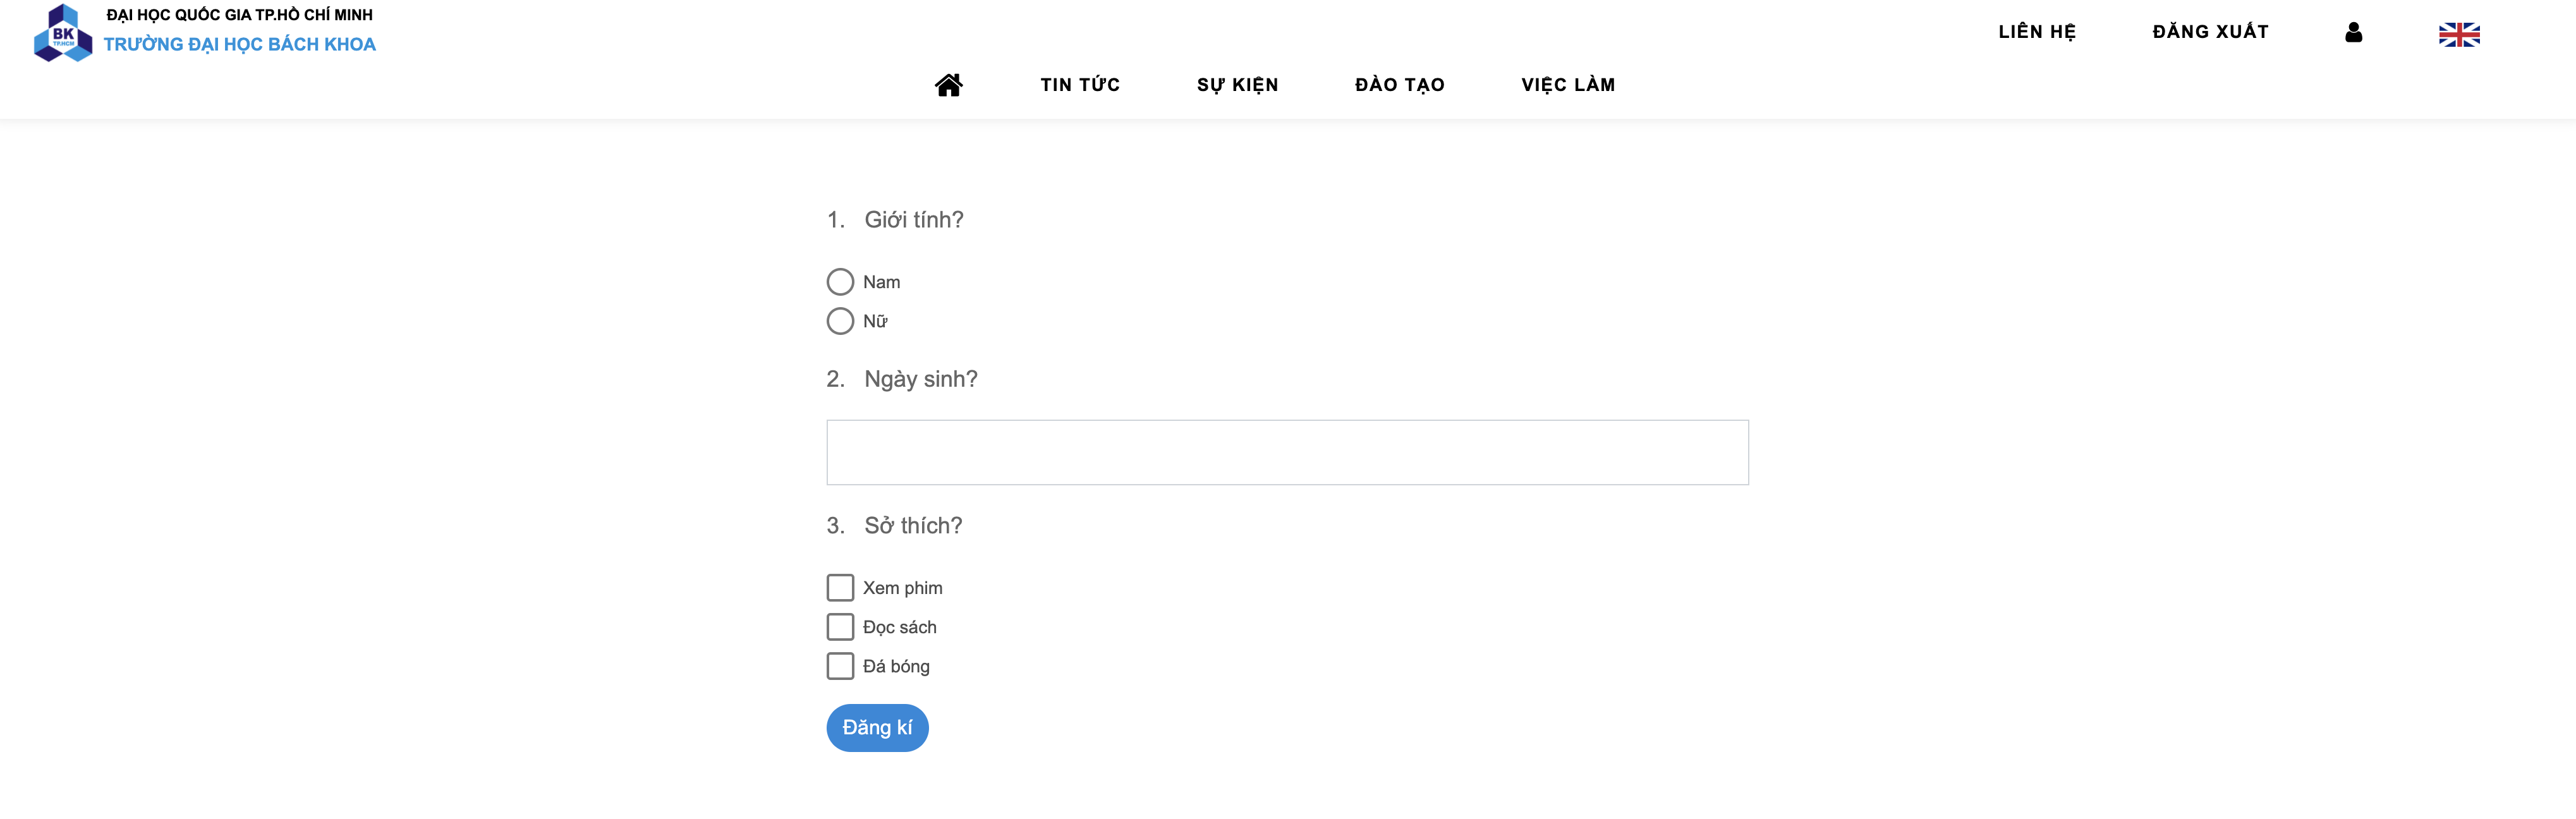
\includegraphics[width=\textwidth]{image/testing-event-register_detail.png}
%   \caption{Giao diện chi tiết đăng ký sự kiện}
%   \label{fig:eventRegisterDetail}
% \end{figure}

% \clearpage
% Khi có danh sách sinh viên tham gia sự kiện, quản trị viên hoặc người điểm danh có thể điểm danh sinh viên tham gia, quá trình này diễn ra đồng bộ, tức thời. Có thể theo dõi danh sách 
% tham gia trực tuyến. Có thể nhiều người điểm danh cùng lúc. Hình \ref{fig:eventRoll} mô tả giao diện điểm danh của quản trị viên.
% \begin{figure}[H]
%   \centering
%   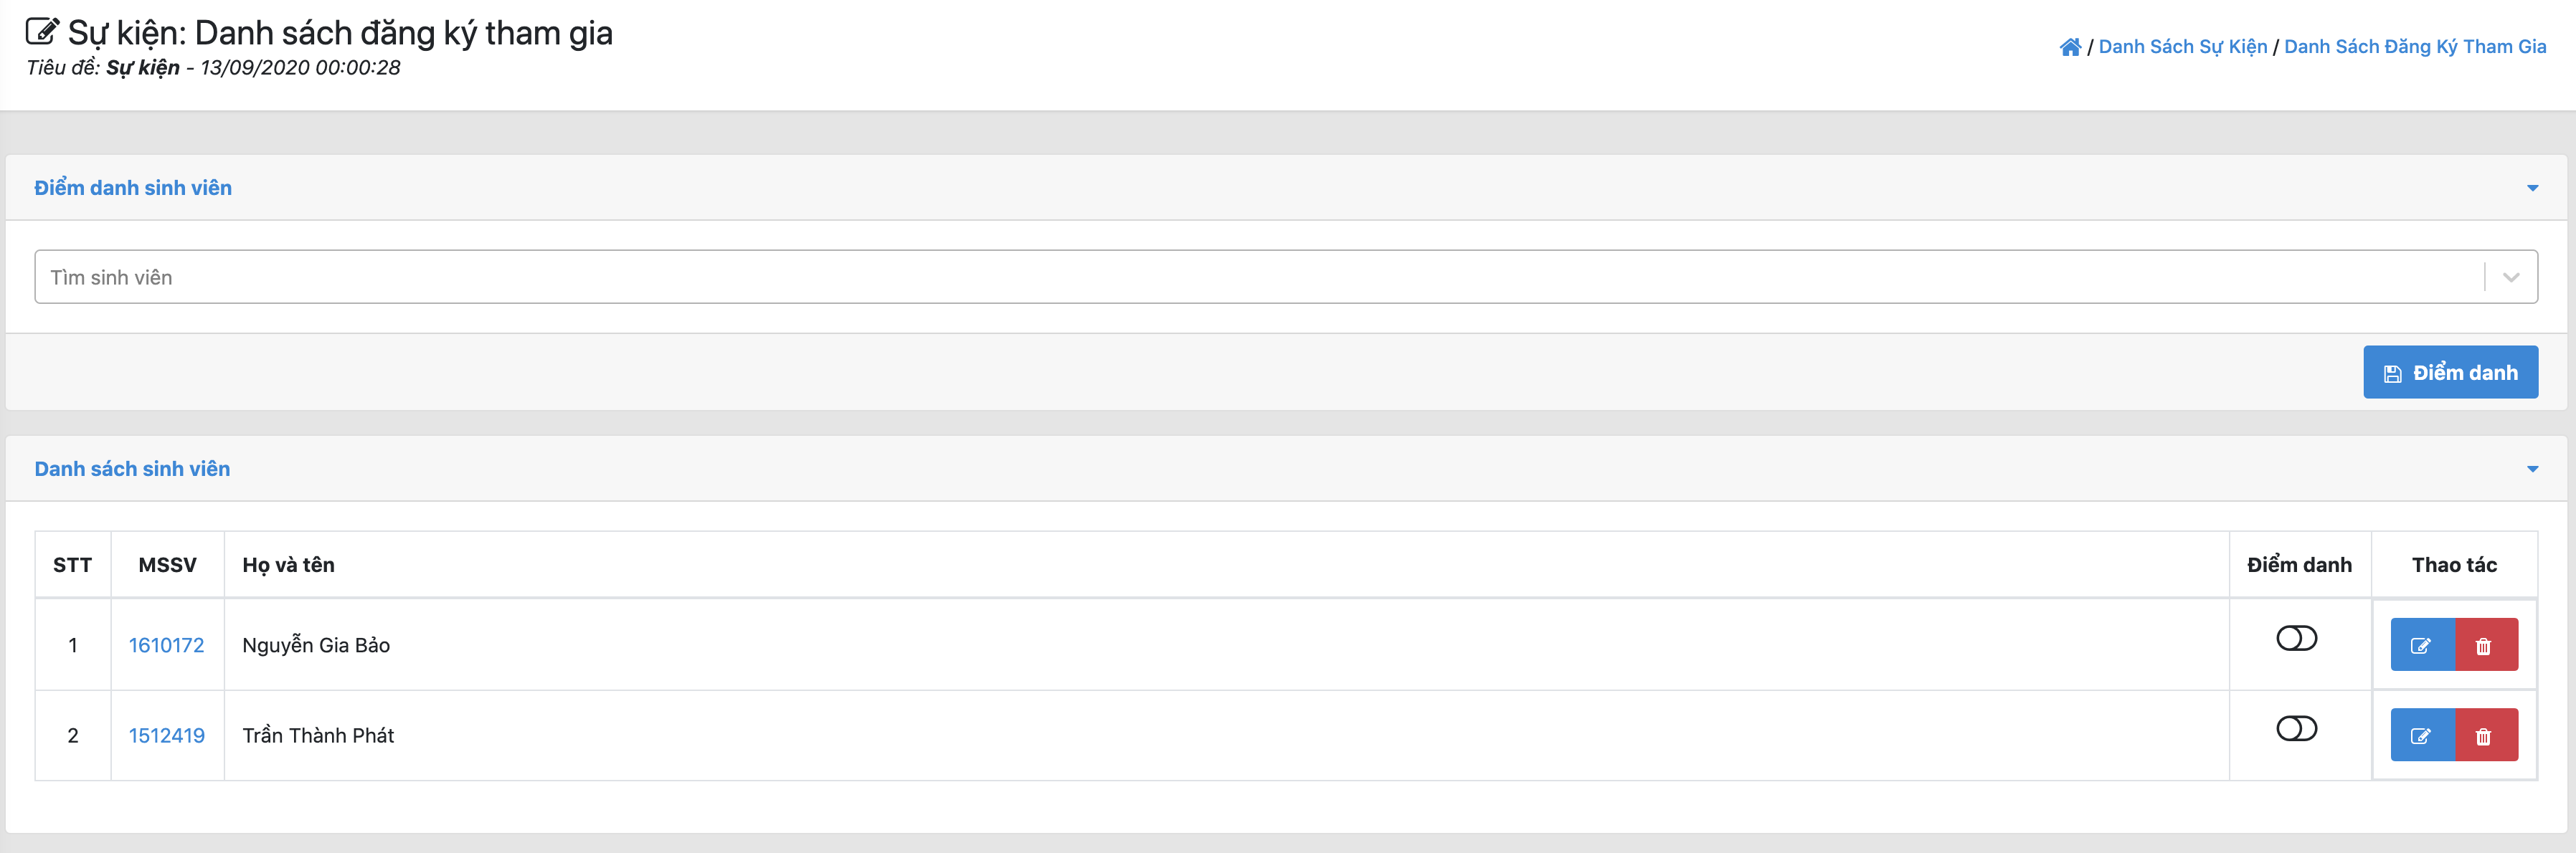
\includegraphics[width=\textwidth]{image/testing-event-register-roll.png}
%   \caption{Giao diện trang đăng ký sự kiện}
%   \label{fig:eventRoll}
% \end{figure}
% \section{Kiểm tra chấp nhận (Acceptance test)}
% Kiểm thử chấp nhận là tiến trình kiểm thử khả năng chấp nhận của chương trình. Mục tiêu là dánh giá sự tuân thủ của hệ thống với các yêu cần nghiệp vụ. Mức kiểm thử này được người sử dụng kiểm thử.

% Bản kiểm thử phần mềm được đưa ra ở sự kiện Jobfair Khoa Máy Tính. Nhằm kiểm thử tính năng tạo và tổ chức sự kiện cho khoảng 1000 sinh viên tham gia.

% Bản kiểm thử thứ hai được đưa ra vào khoảng tháng 04/2021 nhằm kiểm thử tính năng chấm điểm rèn luyện cho sinh viên cuối năm học.
